\begin{enumerate}
	\item Exercício
	
	Calcule o volume do sólido limitado pelos planos:
	\begin{equation*}
		x = 0,\, y = 0,\, z = 0 \textrm{ e } 6x + 2y + 3z = 6
	\end{equation*}
	
	\begin{figure}[htb]
		\caption{Integrais duplas - Aula 10 - Exercício I}
		\label{v10_a10_e01}
		\centering
		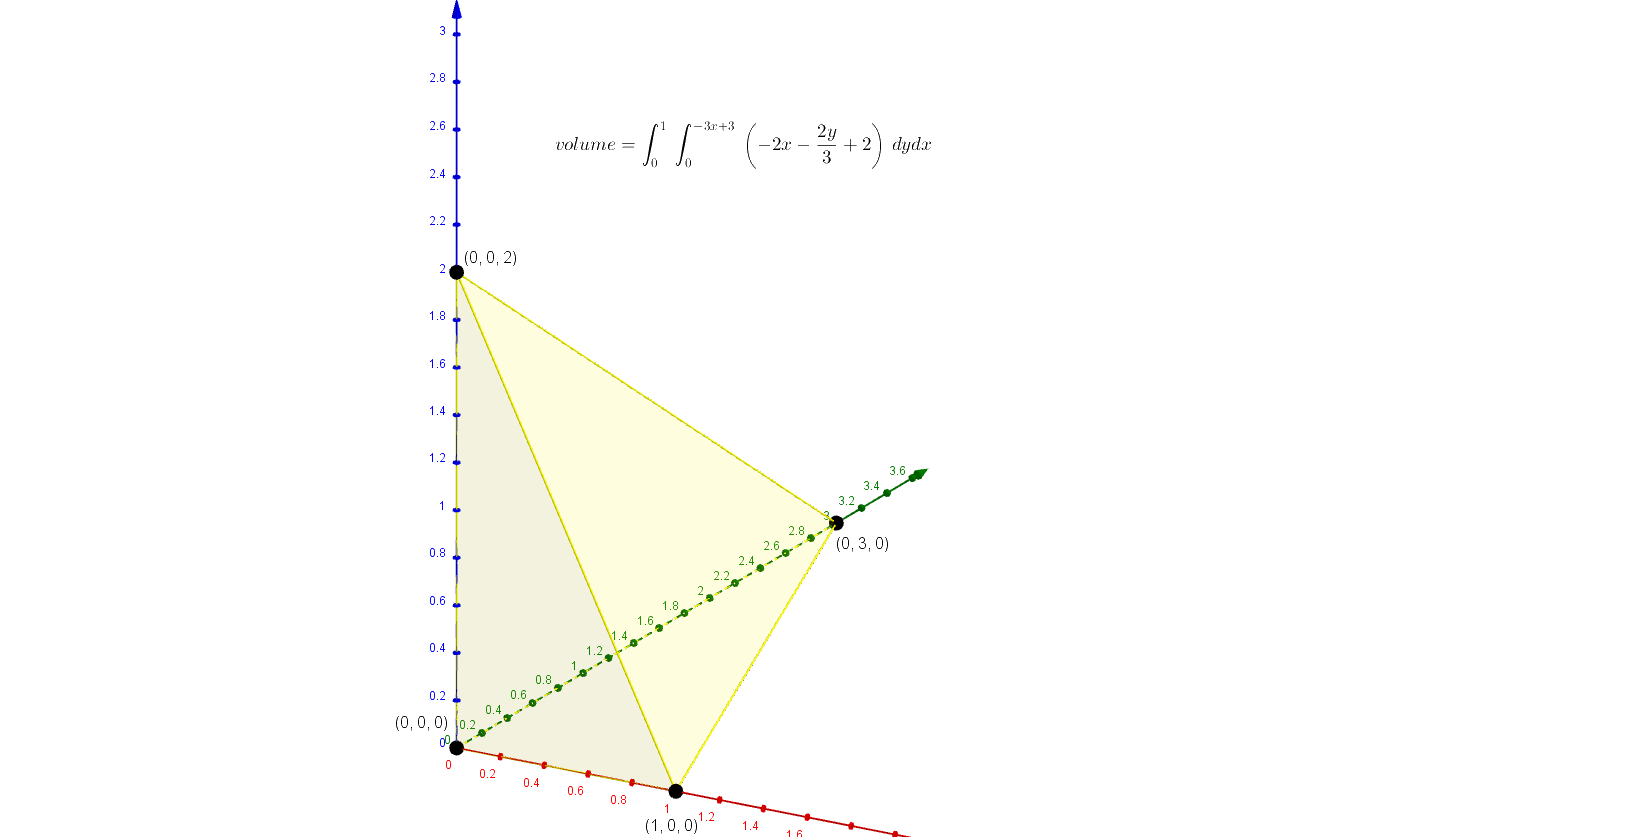
\includegraphics[width=0.5\textwidth]{v10_a10_e01.png}		
	\end{figure}
	
	\begin{equation*}
		P_1 = (0, 0 , 0)	
	\end{equation*}
	\begin{equation*}
		6x = -2y - 3z + 6 \Rightarrow x = \dfrac{-2y - 3z + 6}{6} = \dfrac{-2\cdot0 - 3\cdot0 + 6}{6} = \dfrac{6}{6} = 1 \Rightarrow P_2 = (1,0,0)
	\end{equation*}
	\begin{equation*}
		2y = -6x - 3z + 6 \Rightarrow y = \dfrac{-6x - 3z + 6}{2} = \dfrac{-6\cdot0 - 3\cdot0 + 6}{2} = \dfrac{6}{2} = 3 \Rightarrow P_3 = (0,3,0)
	\end{equation*}
	\begin{equation*}
		3z = -6x - 2y + 6 \Rightarrow z = \dfrac{-6x - 2y + 6}{3} = \dfrac{-6\cdot0 - 2\cdot0 + 6}{3} = \dfrac{6}{3} = 2 \Rightarrow P_4 = (0,0,2)
	\end{equation*}
	\begin{equation*}
		x = 0, x = 1
	\end{equation*}
	\begin{equation*}
		y = 0,\, y = \dfrac{-6x - 3z + 6}{2} = \dfrac{-6x - 3\cdot0 + 6}{2} = -3x + 3
	\end{equation*}
	\begin{equation*}
		z = \dfrac{-6x - 2y + 6}{3} = -2x - \dfrac{2y}{3} + 2
	\end{equation*}
	\begin{align*}
		v = \int_0^1 \int_0^{-3x + 3} \left(-2x - \dfrac{2y}{3} + 2\right)\, dx dy = \int_0^1 dx \int_0^{-3x + 3} \left(-2x - \dfrac{2y}{3} + 2\right)\, dy =\\ \int_0^1 dx\, \left[-2xy - \dfrac{\overstrike{2}}{3}\dfrac{y^2}{\overstrike{2}} + 2y\right]_0^{-3x + 3} = \int_0^1 dx\, \dfrac{1}{3}\left[-6xy - y^2 + 6y\right]_0^{-3x + 3} =\\ \dfrac{1}{3}\int_0^1 dx\, \left[-y(6x + y - 6)\right]_0^{-3x + 3} =\\ \dfrac{1}{3}\int_0^1 dx\, \left[-(-3x + 3)(6x + (-3x + 3) - 6) \overstrike{+ 0(6x + 0 - 6)}\right] =\\ \dfrac{1}{3}\int_0^1 dx\, \left[(3x-3)(3x - 3)\right] = \dfrac{1}{3}\int_0^1 \left(9x^2 - 18x + 9\right) dx = \dfrac{1}{3}\left[9\dfrac{x^3}{3} - 18 \dfrac{x^2}{2} + 9x\right]_0^1 =\\ \dfrac{1}{3} \left[3x^3 - 9x^2 + 9x\right]_0^1 = \dfrac{1}{\overstrike{3}} \left[\overstrike{3}x\left(x^2 - 3x + 3\right)\right]_0^1 =\\ \left[1\left(1^2 \overstrike{- 3\cdot1 + 3}\right) \overstrike{- 0\left(0^2 - 3\cdot0 + 3\right)}\right] = 1	
	\end{align*}
\end{enumerate}